\documentclass[11pt,letterpaper]{article}
\usepackage[T1]{fontenc}
\usepackage[utf8]{inputenc}
\usepackage{lmodern,microtype,amsmath,booktabs,tabularx,longtable,graphicx}
\usepackage[margin=0.8in,headheight=15pt]{geometry}
\usepackage{xcolor,fancyhdr,enumitem,xurl}
\usepackage[hidelinks]{hyperref}
\definecolor{Gold}{HTML}{987100}
\setlength{\parindent}{0pt}\setlength{\parskip}{6pt}
\setlist{nosep,leftmargin=*}\emergencystretch=3em
\pagestyle{fancy}\fancyhf{}\fancyhead[L]{\small Follow My Voice}\fancyfoot[R]{\thepage}
\newcommand{\qid}[1]{\par\smallskip\textbf{\texttt{#1}}\par}
\begin{document}
\setcounter{section}{2}
\section{System Description}
Follow My Voice is a gaze-contingent voice guidance system that helps a seated user find a target object in a surrounding search scene. The system divides responsibility between a local guidance layer, which owns all spatial reasoning, and a cloud language model agent, Jev, which decides how and when to speak. Figure~\ref{fig:architecture} summarizes the pipeline from sensing to speech output. This division keeps task-critical decisions deterministic and auditable while allowing the agent to adapt the phrasing and timing of guidance to the user's recent behavior.

\subsection{Apparatus}
The application is developed in Unity 6 (6000.3.10f1) using the Unity OpenXR Plugin (1.16.1), HTC VIVE OpenXR integration (2.5.1), and Unity XR Interaction Toolkit (3.3.1). It is deployed as a standalone Android ARM64 application on the HTC VIVE Focus Vision head-mounted display, with rendering performed locally on the headset using the Universal Render Pipeline (17.3.0). The headset supplies head-pose and eye-gaze tracking, while the tracked right-hand controller supplies pointing and trigger input. Video passthrough supports the mixed-reality view. Network access supports cloud-based agent decisions and voice preparation; it is not used to stream rendered frames from a host computer.

\subsection{Search Task}
The search task takes place in augmented reality using video passthrough in a neutral physical room. Participants sit on a swivel chair and interact using the right controller. Virtual colored geometric objects hang on eight vertical planes anchored along the surrounding walls. Figure~\ref{fig:scene} shows the layout from above. The application holds the target identity, which is withheld from the opening instructions, so participants must rely on voice guidance to locate it. Participants select an object by pointing the controller ray at it and pressing the trigger. Stimulus density and spatial bounds will be frozen for the study release after seated-comfort and ray-selection pilots. For each trial, the system logs object positions, layout seed, wall assignment, and target identity.

\begin{figure}[htbp]\centering
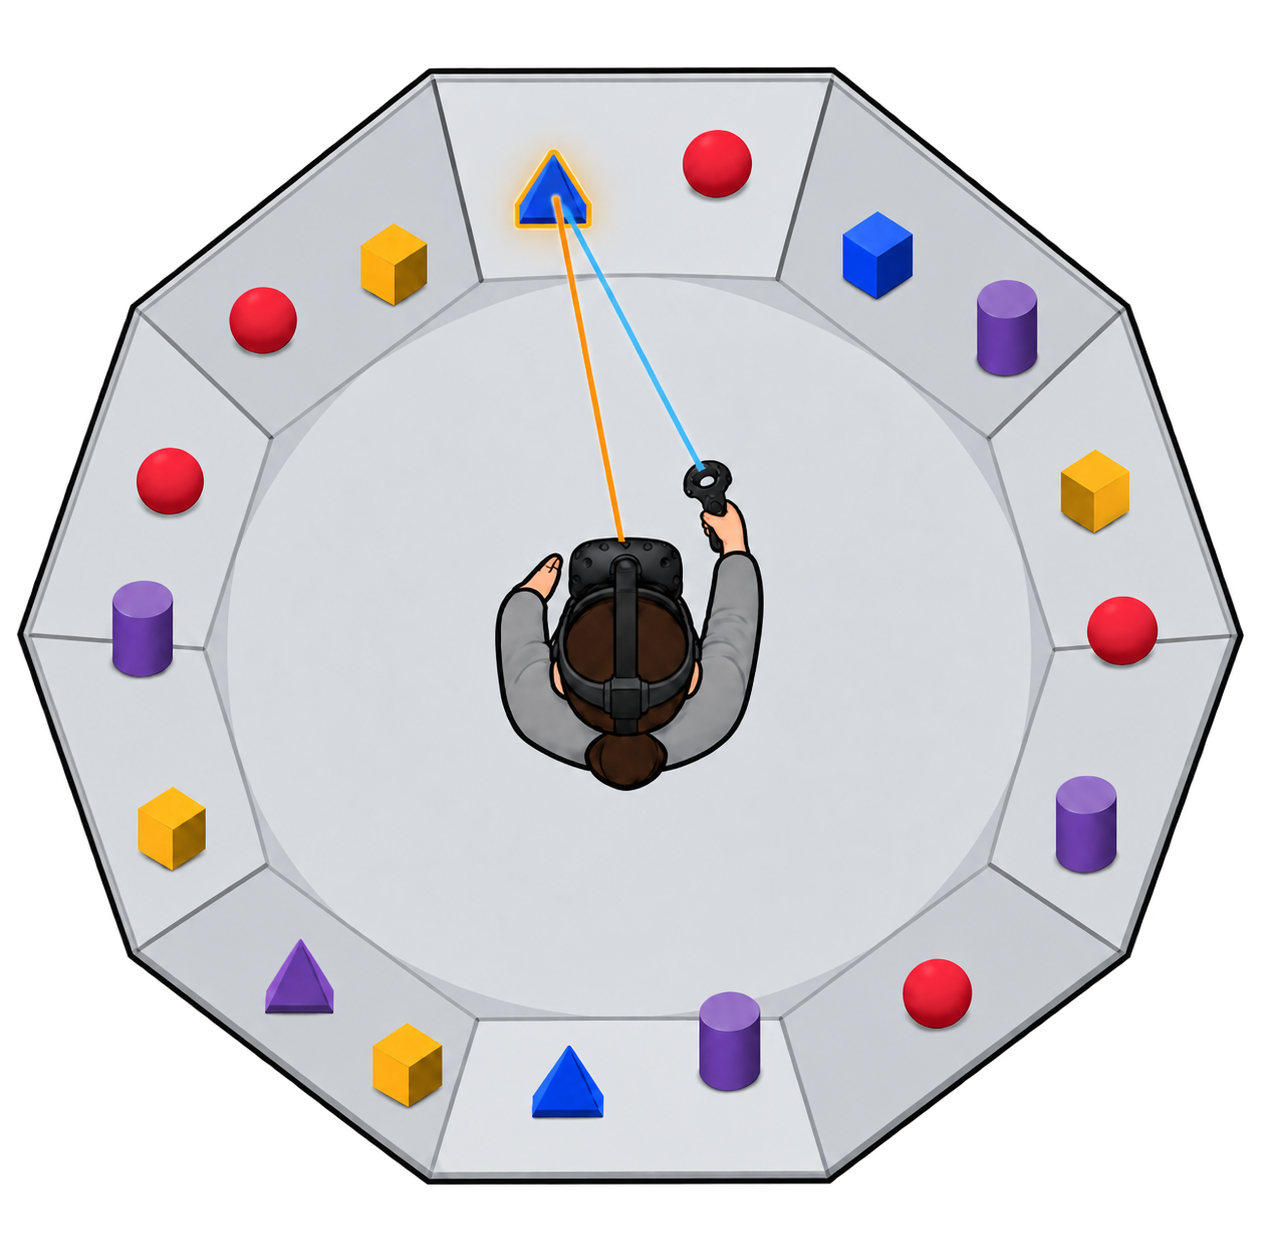
\includegraphics[width=0.6\linewidth]{image.png}
\caption{Top-down view of the search scene. The seated participant is surrounded by wall panels holding colored geometric objects. The gaze ray (orange) and controller ray (blue) converge on the highlighted target, the state in which the participant is ready to select with the trigger. The layout is illustrative; the drawn object count is schematic; object positions and target identity vary by trial.}
\label{fig:scene}
\end{figure}

\subsection{Sensing and Guidance State}
The system continuously collects eye-gaze origin, direction, and validity; head pose; right-controller pose; and ray-object intersections. A local state machine combines these observations with the target geometry to track the participant's progress through the search: turning toward the target wall, refining within the wall, acquiring the target with gaze, pointing with the controller, and becoming ready to select. Additional states cover suspended or paused operation. Each state transition is logged with its cause.

Because guidance is only as reliable as the evidence behind it, the state machine issues new gaze-dependent guidance only when gaze data are valid and recent. Gaze ray hits, gaze-vicinity candidates, and controller hits are treated as separate observations. When gaze-vicinity regions overlap, the closest object is selected. A controller hit immediately suppresses contradictory directional cues, even before the dwell required for spoken pointing confirmation has elapsed, so the system does not direct the participant away from an object they are already pointing at. Gaze confirmation, controller confirmation, and trigger selection are recorded as distinct events.

\subsection{Short-Term Interaction Memory}
To give guidance continuity, the system maintains two short-term memories. A spatial history tracks turning progress and supports cues that return the participant to the target. A speech-decision memory records what the system actually said and how the guidance state changed. Each speech entry stores its relative age, context, and whether playback completed or was interrupted; each state entry stores the prior and current states and the reason for the transition. The speech and transition lists each retain at most four entries; snapshots sent to Jev exclude entries older than 15 seconds. This bounded recent context is related to the context-management motivation of EmBARDiment~\cite{bovo2025embardiment}, but the current implementation does not use its object-admission or dropout policy. The separate spatial history retains up to three seconds or 384 target-relative gaze observations and clears on invalid evidence, source changes, or observation gaps longer than 100~ms. These limits are engineering settings, not validated fixation or blink thresholds. Gaze-vicinity confirmation currently requires 100~ms of valid qualifying evidence; invalid evidence resets its entry timer, and reacquisition after a spoken confirmation requires 150~ms of valid gaze away. Those interaction gates do not admit objects to speech memory, and missing gaze is not counted as observed dwell. The memory is cleared whenever guidance resets and is copied before each asynchronous request. This memory is deliberately scoped to the current task: it does not build a persistent participant profile or attempt to infer unobserved mental states.

\subsection{Agent Decisions and Playback Control}
Jev selects from a constrained set of options rather than generating free-form instructions. Local geometry and state rules first filter the phrase library to candidates that are valid in the current situation. Each request to Jev contains a state snapshot, recent memory, playback status, and two to five eligible phrases. Jev then chooses the wording and whether to speak now or wait. Target definition and geometric reasoning remain local. Eligibility filtering and playback revalidation reduce spatially incorrect or stale guidance, but tracking error, imperfect geometry and software faults can still produce unhelpful instructions; recorded-sequence and headset checks remain necessary.

Because cloud responses arrive asynchronously, the participant's state may change before a decision returns. A local speech scheduler therefore revalidates each decision against the current state, evidence, pacing, and object intersections before playback, and discards decisions that are stale or conflict with the current situation. Feedback that qualifies for local handling is played from prepared phrases without waiting for a new cloud decision, subject to the same checks. Each completed or interrupted utterance updates both the memory and the event log. Model latency, deferral, cancellation, fallback, and playback onset are logged separately, so any delay in speech can be attributed to the stage that caused it.

\begin{figure}[htbp]\centering
\IfFileExists{voice-guidance-memory-architecture.pdf}{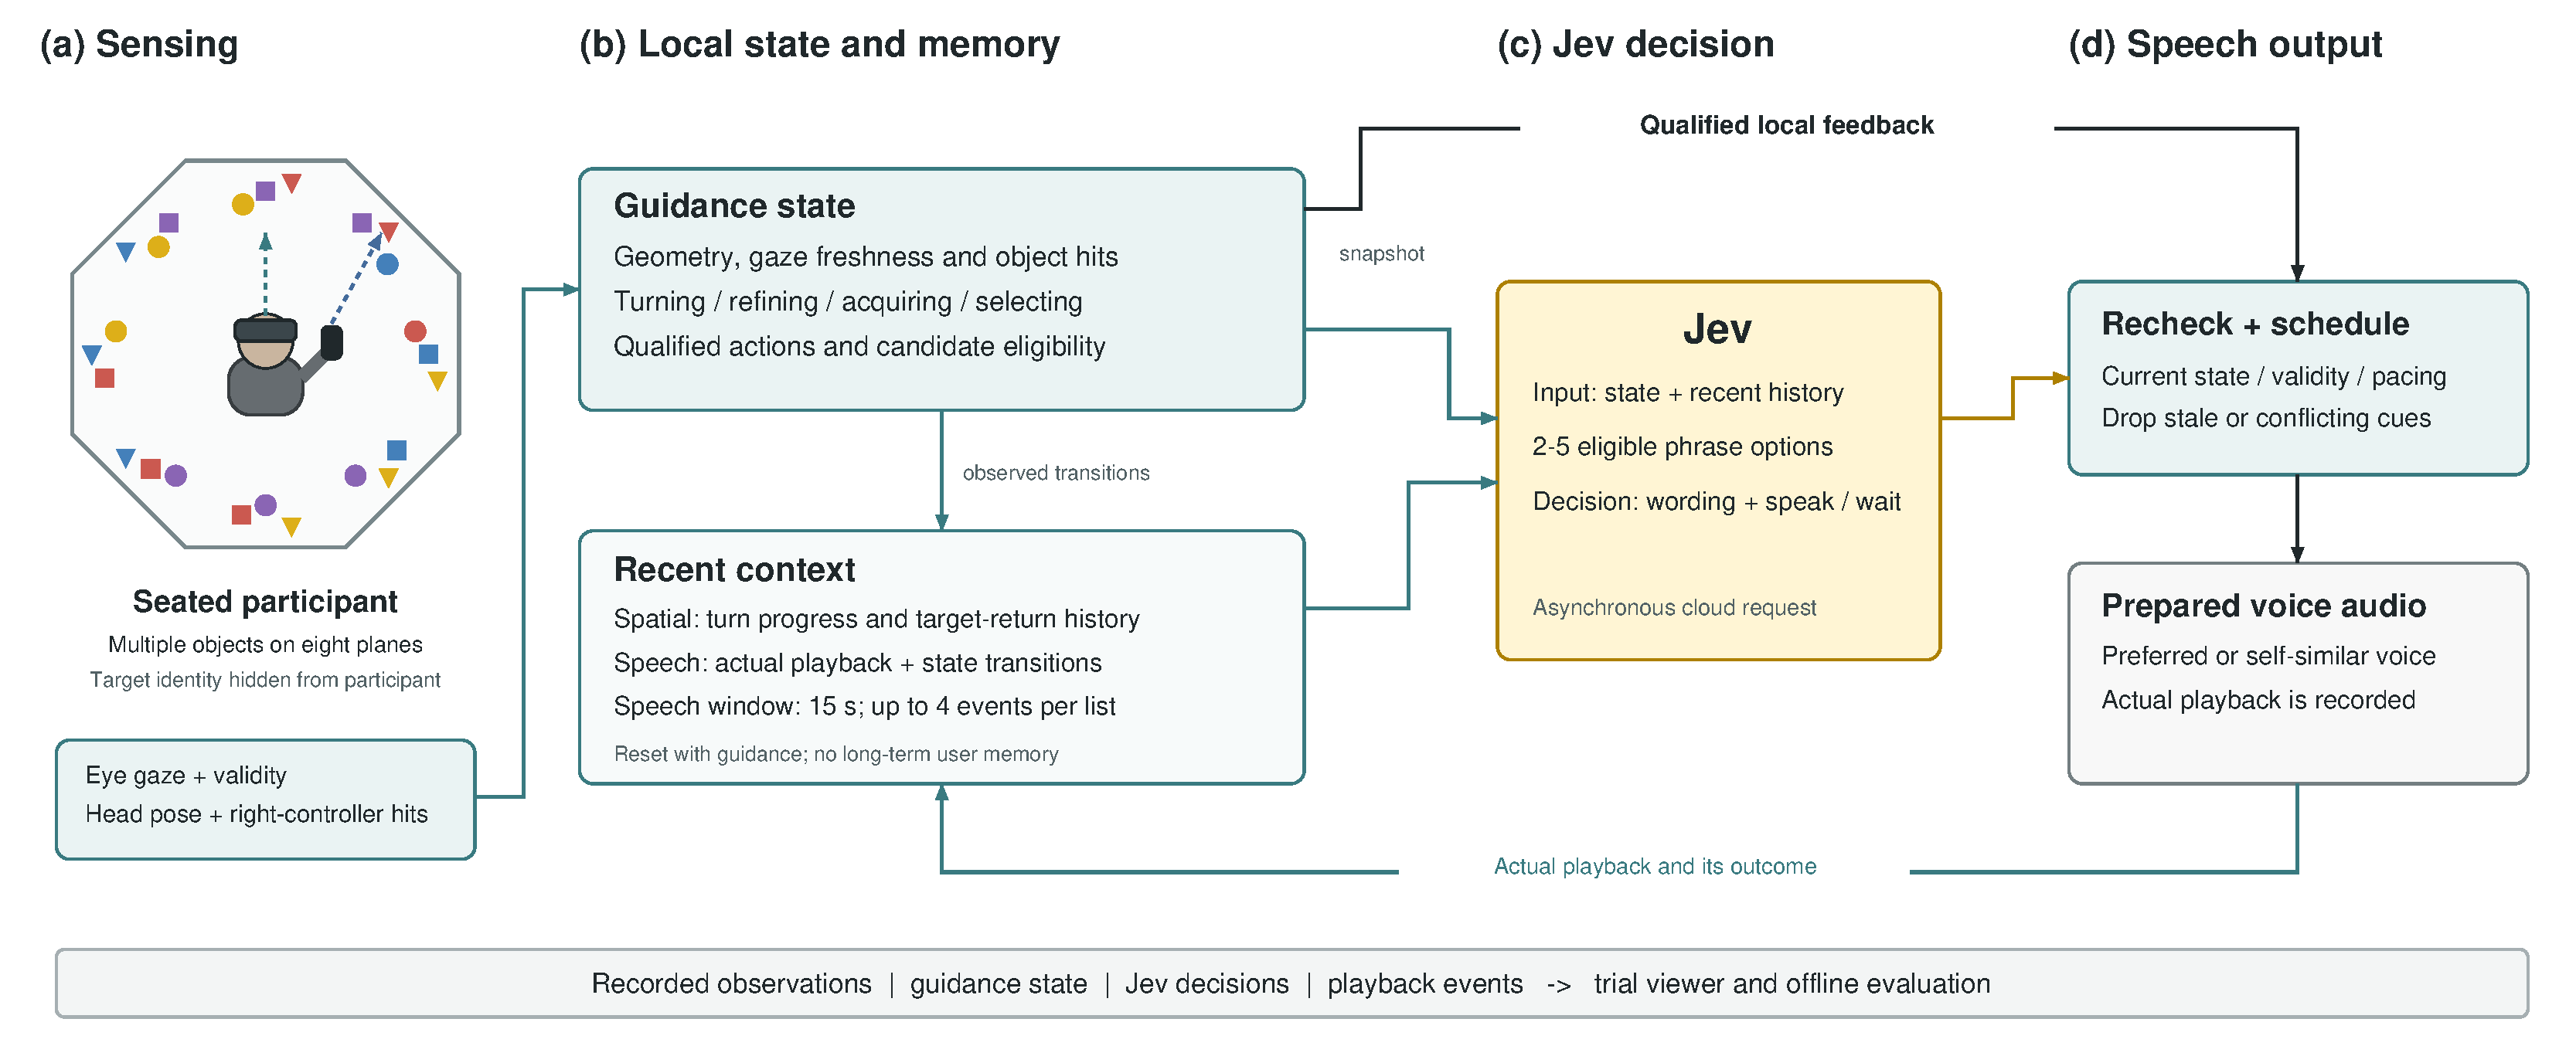
\includegraphics[width=\linewidth]{voice-guidance-memory-architecture.pdf}}{\fbox{\parbox{0.94\linewidth}{Gaze and controller observations $\rightarrow$ local state and bounded context $\rightarrow$ eligible choices for Jev $\rightarrow$ current-state recheck $\rightarrow$ prepared voice playback. Qualified local feedback also enters the recheck stage.}}}
\caption{System architecture. (a) Gaze, head, and controller data are sensed. (b) A local state machine and short-term memory determine which guidance actions are valid. (c) Jev chooses wording and timing from eligible options. (d) The scheduler revalidates each cue against the current state before playback. Actual playback feeds back into memory. The scene inset is schematic and does not reflect stimulus count or any participant-visible target cue.}
\label{fig:architecture}
\end{figure}

\subsection{Voice Preparation and Telemetry}
All voice audio is pre-synthesized with ElevenLabs, which supplies both the catalog voice and the self-similar voice. To support the self-similar condition, each participant records the same standard passage in their usual speaking voice. Both conditions share the semantic phrase library, guidance policy, and playback routing. Voice condition is the intended manipulation; behavior-dependent wording, hint counts and synthesized acoustics need not be identical. The preparation pipeline checks wording and library readiness. Per-voice intelligibility, loudness and acoustic comparability still require pilot verification; automated checks do not establish perceptual equivalence. No pitch or spatial effects are applied to the self-similar voice. We log the provider, model, voice ID, library version, and synthesis settings.

A trial viewer aligns gaze and controller state, guidance transitions, agent decisions, and playback events with trial geometry on a common timeline. Trial-level aggregates are stored separately from the raw gaze, motion, and event streams. Effective gaze sampling rate must be verified from distinct source timestamps on the tested headset build rather than inferred from the nominal specification or application polling rate. Similarly, we report ray intersections as gaze hits and do not label them as fixations unless a validated event classifier is applied.
\bibliographystyle{plain}
\bibliography{references}
\end{document}
